\logvartrue
\chapter{Appendix 1}

\section[Evolution of intra-specific regulatory networks in a multipartite bacterial genome]{Evolution of intra-specific regulatory networks in a multipartite bacterial genome%
\sectionmark{Evolution of intra-specific regulatory networks}}
\sectionmark{Evolution of intra-specific regulatory networks}

The gene regulatory network is an important step in the understanding of how organisms precisely control the expression of gene products and therefore phenotypes. Recent studies have pointed out the importance of regulatory networks plasticity in bacterial adaptation and evolution. The evolution of such networks within and outside the species boundary is still obscure though. \textit{Sinorhizobium meliloti} is an ideal species for such study, having three large replicons, many genomes available and a significant knowledge of its TFs. Each replicon has a specific functional and evolutionary mark which might also emerge from their regulatory signature.\\
Here we study the plasticity of the regulatory network within and outside the \textit{S. meliloti} species, looking for the presence of 41 TFs binding motifs in 51 strains and 5 related rhizobial species. We detected preference of several TFs for one of the replicons, and the function of regulated genes was in accordance with the overall replicon functional signatures: house-keeping functions for the chromosome, metabolism  for the chromid, symbiosis functions for the megaplasmid, thus suggesting a replicon-specific wiring of the regulatory network in the \textit{S. meliloti} species. At the same time a significant part of the predicted regulatory network is shared between the chromosome and the chromid, thus adding an additional layer by which the chromid integrates itself in the core genome.\\
Furthermore, the regulatory network distance was found to be correlated with both promoter regions and dispensable genome evolution inside the species, indicating that both pangenome compartments are involved in the regulatory network evolution. Indeed, genes of the dispensable regulon missing both a TFBS and its cognate TF were shown to likely belong to the dispensable genome, possibly due to the relaxation of selective constraints. Regulatory interactions should then also be considered to predict evolutionary conservation and dynamics in bacterial pangenomes.\\

% Please keep the Author Summary between 150 and 200 words
% Use first person. PLoS ONE authors please skip this step. 
% Author Summary not valid for PLoS ONE submissions.   
\subsection*{Author Summary}
The influence of transcriptional regulatory networks on the evolution of bacterial pangenomes has not yet been elucidated, even though the role of transcriptional regulation is widely recognized. Using the model symbiont \textit{Sinorhizobium meliloti} we have predicted the regulatory targets of 41 TFs in 51 strains and 5 other rhizobial species, showing a correlation between regulon diversity and pangenome evolution, through upstream sequence diversity and dispensable genome composition. We have also shown that genes not wired to the regulatory network are more likely to belong to the accessory genome, thus indicating that regulation imposes a selective constraint on bacterial pangenomes evolution. We have also highlighted a series of TF that preferentially regulate genes belonging to one of the three replicons of this species, indicating the presence of replicon-specific regulatory modules, with peculiar functional signatures. At the same time the chromid shares a significant part of the regulatory network with the chromosome, indicating an additional way by which this replicon integrates itself in the pangenome.\\

\subsection{Introduction}
Regulation of gene expression is recognized as a key component in the cellular response to the environment. This is especially true in the bacterial world, for two reasons: bacterial cells are often under severe energy constraints, the most important being protein translation \cite{depardieu2007modes} and they usually face a vast range of environmental and physiological conditions; being able to efficiently and readily react to such conditions can most certainly give a selective advantage over competitors.\\
Transcription is mainly regulated by proteins, called transcription factors (TF), which usually contain a protein domain capable of binding specific DNA sequences, called TF binding sites (TFBS). Depending on the position of the TFBS with respect to the start codon of the regulated gene, the transcription factor can act either as an activator or a repressor of transcription, mostly because of its interaction with the RNA polymerase and its sigma factors \cite{gruber2003multiple, van2009mechanisms}. The binding of the TF to its cognate TFBS is based on non-covalent interactions whose strength is indicated by the so-called affinity constant. Since TFBS can have variations around a preferred sequence, the affinity of a TF for its TFBSs covers a continuous range of values; however, since the TF binding strength appears to follow a sigmoid behaviour, it is possible to distinguish between 'weak' and 'strong' TFBSs \cite{lassig2007biophysics}.\\
As opposed to eukaryotic species, prokaryotic TFBS are usually distinguishable from the 'background DNA', and they tend to have a simpler structure and a close proximity to the transcription start site \cite{wunderlich2009different}. The application of information theory concepts to TFBS has highlighted the dependency of the TF binding specificity to the so called information content of its TFBS, which depends on its length, variability and composition with respect to the overall genomic background (i.e. the sequence composition). The minimum information content for a TF motif to be specifically recognizable intuitively depends on the genome size and genome composition: in a large genome the probability of a false positive is larger and much larger if the composition of the TFBS is close to the background DNA composition. Transcription factors with low information content TFBS usually control the transcription along the whole genome, such as alternate sigma factors and also show a larger variability between species \cite{quinn2014bacterial}; the gene targets of these TFs are also harder to reliably predict, for the presence of many putative site along the whole genome. Bacterial TFs are also usually encoded in the proximity of their targets; their orientation with respect to the regulated genes can also be used to infer whether the TF acts with a positive or negative interaction \cite{janga2007internal, westholm2008genome}. The high gene density of bacterial genomes and its organization in operons results in the expression or repression of whole functional pathways in response to stimuli, again highlighting the influence of cellular energy constraints. Furthermore, the presence of several TFBS in the upstream region of a gene can result in a complex transcriptional response that recall logic gates \cite{hunziker2010genetic}.\\
Prediction of TFBSs in a genome usually relies on the availability of a position specific scoring matrix (PSSM) storing the frequency of each nucleotide at each position of known TFBSs. PSSM modeling the variability of a TFBS can be built by identifying enriched DNA patterns in promoter regions of genes that are known to be under the control of the TF under analysis, or through other assays like the binding of the TF to synthetic nucleotides. Several algorithms have been developed to use such PSSM to search for TFBS in nucleotide sequences, such as the MEME suite \cite{bailey2009meme}, RSAT \cite{van2003regulatory, thomas2008rsat, thomas2011rsat} and the Bio.motif package \cite{cock2009biopython}; a recent alternative method relies on the construction of a hidden markov model (HMM) from an alignment of nucleotide sequences, which can then be searched inside a query nucleotide sequence \cite{eddy2009new, johnson2010hidden, eddy2011accelerated}. Since all these methods and their different implementations have different weaknesses, it has been advised to use a combination of those methods in a search of TFBS inside a genome \cite{harbison2004transcriptional}.\\ 
Regulatory networks in bacteria evolve rapidly, making the comparisons between distant organisms difficult \cite{babu2006evolutionary, gelfand2006evolution, janga2007structure, lozada2006bacterial}. At broad phylogenetic distances, it has been shown that the conservation level of a TF is lower than the one of its targets, but also that species with similar lifestyles tend to show conservation of regulatory network motifs, despite significant variability in the gene composition of the network, suggesting an evolutionary pressure towards the emergence of certain regulatory logics \cite{babu2006evolutionary}.\\
The fluidity of most transcriptional regulatory connections is well known and documented not only at large phylogenetic distances, but at the level of intra-species comparisons too \cite{hendriksen2007regulation, brilli2010diversity, frandi2010comparative, galardini2011exploring}. 
Experiments have shown that Bacteria have high tolerance towards rewiring of regulatory circuitry and, then, they can possibly exploit radical changes in regulatory targets, without extensive changes in phenotypes \cite{isalan2008evolvability}. At the same time, examples where a single change in the regulatory network results in a change in phenotype have been reported \cite{somvanshi2012single, blount2012genomic}. Consequently, there is a large evolutionary potential in bacteria provided by the plasticity of both the genome and its regulatory circuitry. The extent of variability and evolution of the regulatory network inside a species is however still poorly understood.\\
The aim of this study is to apply a comparative genomics approach to regulatory network predictions, deciphering the impact of the regulatory network variability on pangenome evolution. We decided to use the \textit{Sinorhizobium meliloti} species, the nitrogen-fixing symbiont of \textit{Medicago} plants, for which an extensive knowledge on TF is present in the literature \cite{krol2011rhizoregnet, schluter2013global}. This species presents a marked genomic difference with respect to well-know model species, as \textit{Escherichia coli}, since the genome comprises three main replicons of comparable size: a chromosome, a chromid \cite{harrison2010introducing} and a megaplasmid, each one with distinct functional and evolutionary signatures \cite{galibert2001composite, galardini2013replicon}, raising the question if the evolution of the regulatory network may be influenced by functional and evolutionary differences among replicons. Recent reports have shown that there are only two genes essential for growth in minimal media and soil encoded in the \textit{S. meliloti} chromid\cite{maclean2014examination}, even though the chromid harbours many core genes. Moreover, \textit{S. meliloti} has several genomes sequenced to date \cite{galibert2001composite, galardini2011exploring, schneiker2011complete, li2012draft, sugawara2013comparative, weidner2013genome, martinez2013complete, sallet2013next, Galardini2013sigs} and the potential for biotechnological and agricultural applications, which could benefit from the insights generated from a regulatory network analysis. At the gene level, the pangenome of this species has a significantly large fraction of conserved genes of around 5000 gene families \cite{galardini2013replicon, sugawara2013comparative}.\\
We have therefore constructed the comparative regulatory network of the \textit{S. meliloti} species, using the PSSM of 41 TFs collected from the literature and public databases and applying a combination of TFBS prediction methods, combining this predictions with the information about core and dispensable gene families. We have also predicted the presence of the same TFBS to other five closely related rhizobial species (termed 'outgroups': \textit{Rhizobium leguminosarum} bv. \textit{viciae}, \textit{Rhizobium etli}, \textit{Mesorhizobium loti}, \textit{Sinorhizobium fredii} and \textit{Sinorhizobium medicae}), in order to highlight the different behaviours that are present within and between species. Our predictions and other comparative genomics observations are publicly available \href{https://github.com/combogenomics/rhizoreg/tree/paper}{here}.\\

% Results and Discussion can be combined.
\subsection{Results}

\subsubsection{General features of the predicted regulatory network of \textit{S. meliloti}}
As the variable component of the \textit{Sinorhizobium meliloti} pangenome accounts for about 40\% of their proteome size \cite{galardini2013replicon, sugawara2013comparative}, it is reasonable that the same proportion could be also applied to transcription factors (TFs).\\
Based on COG annotations, all the 51 S. meliloti  strains analysed in this study, have been found to encode a similar number of predicted TFs (552 average); a similar number has been also found in the five outgroups (average 533).\\
This is in accordance with previous reports correlating genome size with the number of TFs \cite{charoensawan2010genomic}; alpha-rhizobial genomes, which are known to have larger genomes compared to other bacteria from the same phylum \cite{pini2011plant}, have then the largest collection of TFs in the known bacterial kingdom.\\
About 70\% of all the TFs encoded in the \textit{S. meliloti} pangenome belong to the core genome, while the remaining TFs appear to be singletons in the pangenome, belonging to just one strain or very few (2-3 strains); this orthologous genes distribution is similar to the one observed for the whole pangenome \cite{lobkovsky2013gene} (Figure SM1).\\
 Given the relatively high conservation of TFs in the \textit{S. meliloti} pangenome, most of the 41 TFs analysed in this study were found to be conserved in all strains, the only notable exception being RhrA, the activator of the rhizobactin regulon, which has been found to be absent in 18 strains (35\% of the total). This confirms earlier reports on the variability in presence of this system related to symbiosis \cite{lynch2001genetic, gill1991high, galardini2011exploring}. More interestingly, recent reports have demonstrated how the presence of the rhizobactin operon confers competitive advantage over other \textit{S. meliloti} strains in iron limited environments \cite{maclean2014examination}; we could therefore speculate that a significant fraction of the \textit{S. meliloti} strains have a competitive disadvantage in the absence of iron.\\
 Surprisingly, an ortholog of FixJ (an important symbiosis key regulator) was not predicted in two \textit{S. meliloti} strains (A0643DD and C0438LL), but this could most likely be due to the annotation draft state of these genomes.\\
As expected, more TFs (16) were absent in at least one of the other five outgroups, many of whose orthologs are encoded in the \textit{S. meliloti} symbiotic megaplasmid pSymA (6 TFs out of 9 analysed), including two copies of NodD, FixJ, RctR, SyrM and RhrA (Figure SM1).\\
 Such difference between intraspecific and interspecific TF gene content may anticipate a similar difference at the downstream regulatory network, for the absence of cross-regulatory links.\\
To ensure a high confidence in the TFBS predictions we selected the TF motifs with relatively high information content (see Materials and Methods).\\
We observed a wide range of information gain for TFBSs; of the starting 83 TFBS retrieved from literature and databases, 41 have been found to have enough information content to reliably predict their TFBS (Figure~\ref{fig:reg1} (a), Table SM1).\\%
\begin{figure}[!tb]
	\centering
	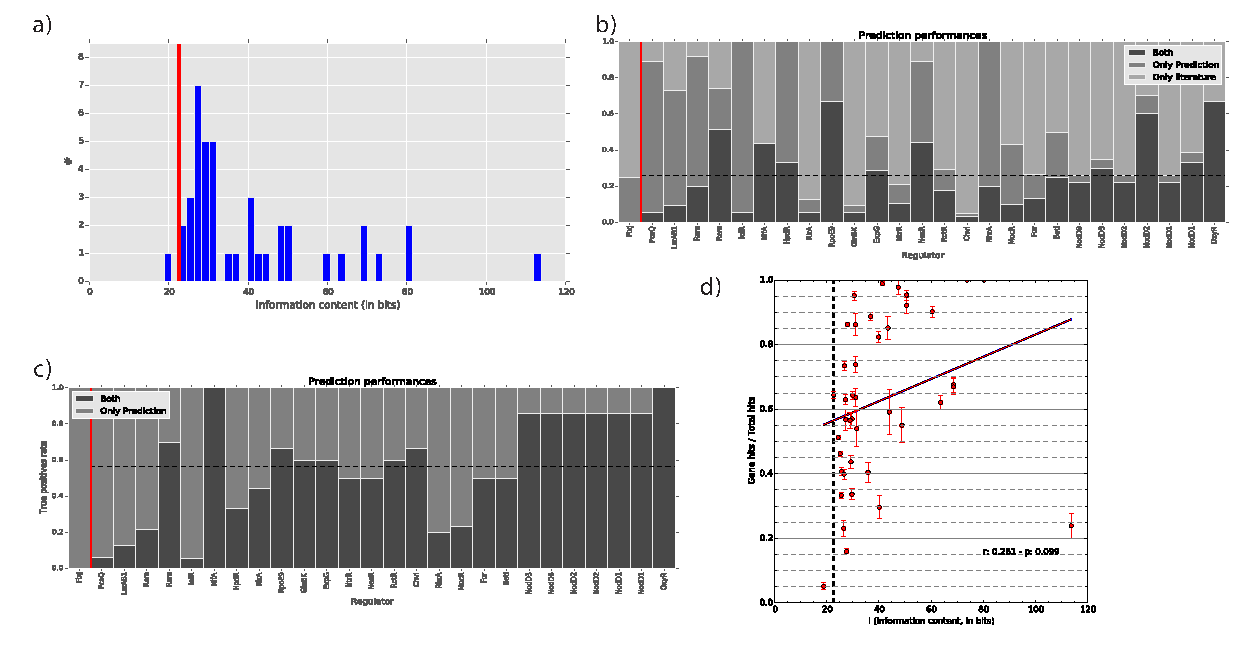
\includegraphics[width=1\textwidth]{./figures/Appendix_1/1_reg}
  	\caption{\label{fig:reg1} General characteristics of the presented TF predictions and quality control. a) Information content frequencies for the 41 analysed TFs: vertical line indicates the minimum information content, as measured for \textit{S. meliloti} strain Rm1021; b-c) comparison between TFBS predictions and the reported experimental results in strain Rm1021: the dashed horizontal line indicates the mean value for the TFs with information content higher than the minimum value; d) correlation between the TFs information content and the signal-to-noise ratio: vertical bars indicate the error level measured in all the strains.}
\end{figure}%
For FixJ two separate motifs acting together have been described \cite{ferrieres2002two}, one above and one slightly below the threshold: both motifs have been used.\\
We applied a novel TFBS prediction approach to overcome common problems associated with the prediction algorithms and maximize accuracy and sensitivity \cite{van2009mechanisms}, including operon predictions to recover most of the downstream regulated genes (see Materials and methods).\\
 The predictions accuracy was determined with a comparison with the downstream regulons reported in the literature, when available (Figure~\ref{fig:reg1} (b and c)); the average accuracy of the predictions was found to be around 55\%, with a tendency to positively correlate with the motif information gain (Figure SM2).\\
On the other hand, a relatively high number of downstream genes were predicted only in the literature.\\
This behaviour may be explained by the fact that most regulons have been defined on the basis of gene expression data; since these experiments are not focused on genes directly under the control of a specific TF, many targets can be regulated by TFs which are downstream in the regulatory cascade and therefore cannot be predicted by our search strategy.\\
Predicted TFBS in genes upstream regions against TFBS predicted in coding regions were considered a signal to noise ratio (upstream hits on total hits) to measure the predictions quality (Figure~\ref{fig:reg1} (d)); for more than 70\% of the analysed TF the observed ratio was above 50\%, with a very poor correlation with the motif information content.\\
Taken together these results show that our predictions are of fairly good quality. We further experimentally confirmed some of the predictions on a subset of predicted promoters of the NodD regulon (Table SM2).\\%
\begin{figure}[!tb]
	\centering
	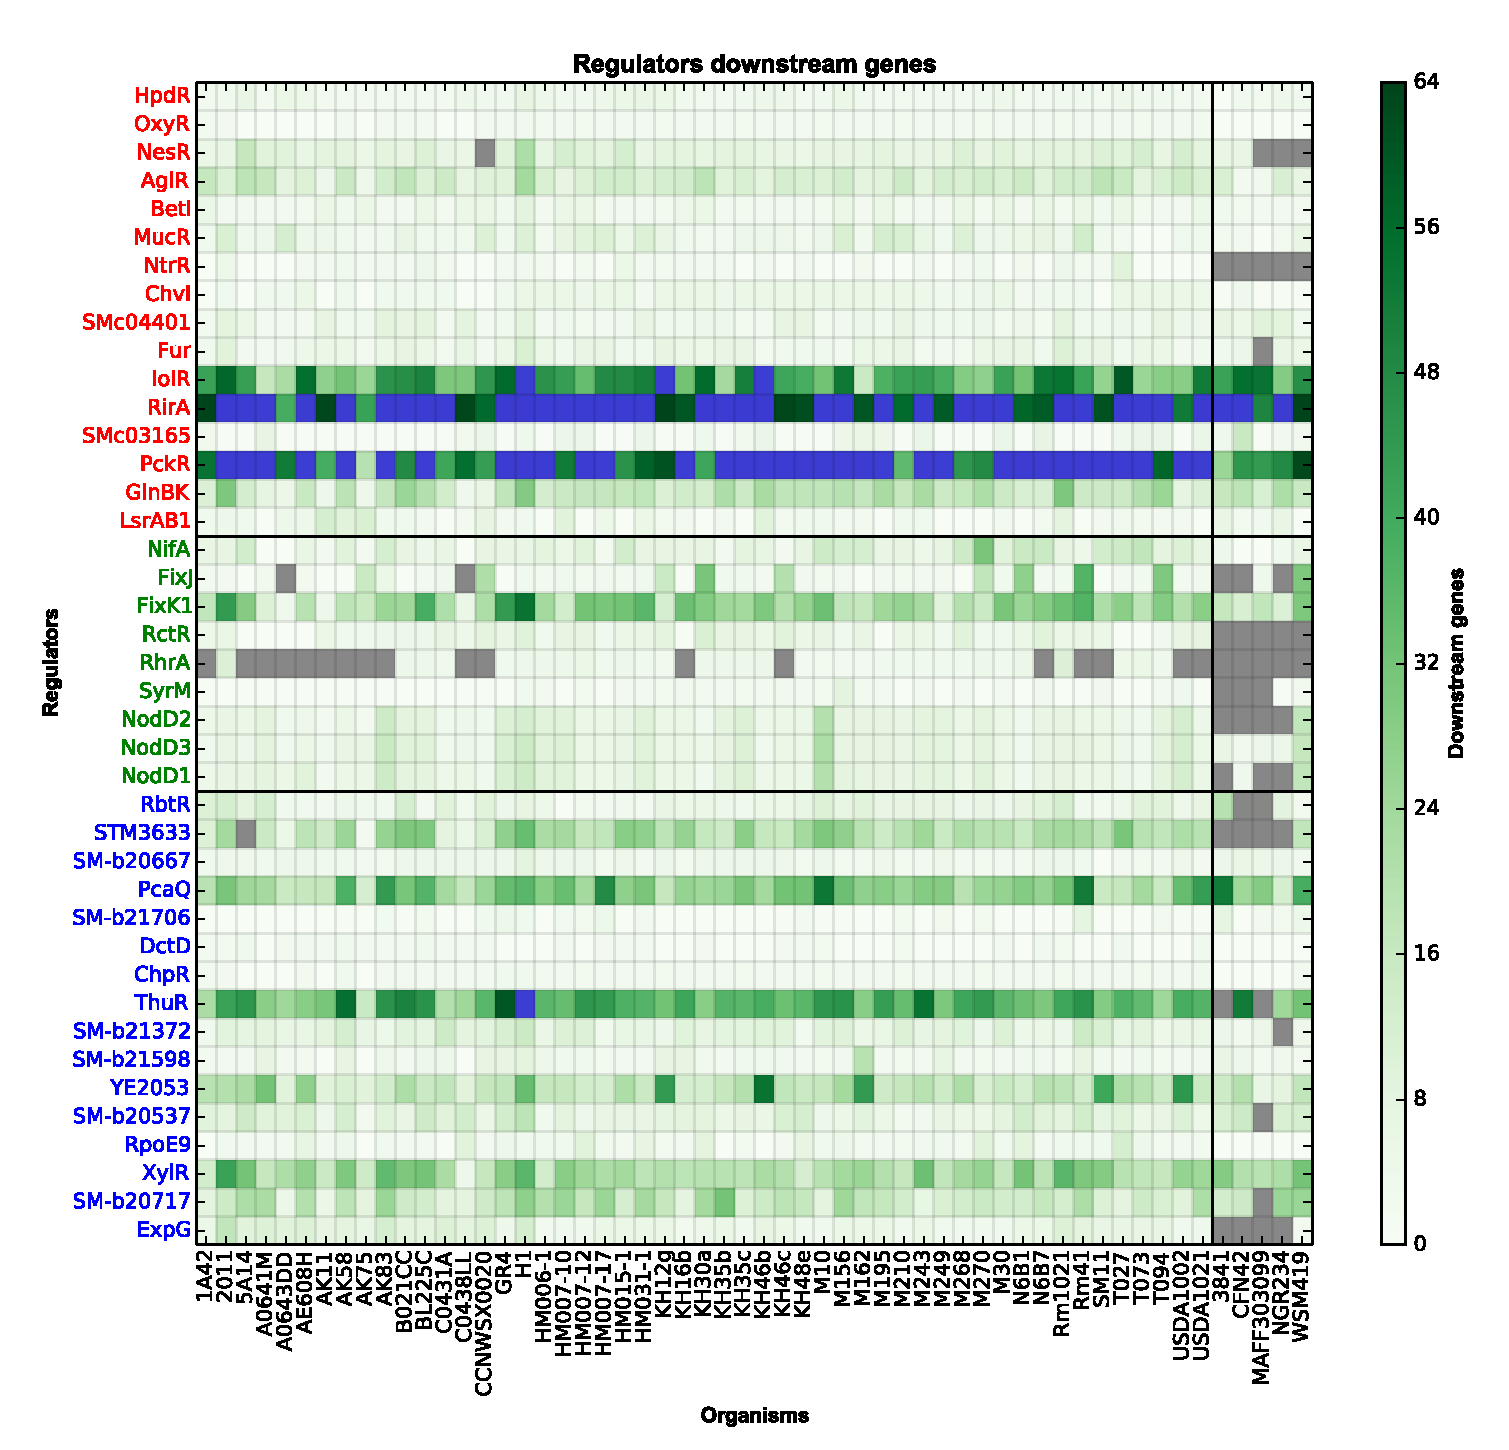
\includegraphics[width=0.7\textwidth]{./figures/Appendix_1/2_reg}
  	\caption{\label{fig:reg2} Variability in regulon size. Color intensity indicates the number of downstream regulated genes in each strain; gray squares indicate the TF absence in the genome of that particular strain. Blue squares indicate that there are more than 64 genes predicted to be under the control of the TF. TFs are colored according to the replicon they belong to: red for chromosome, green for the pSymA megaplasmid and blue for the pSymB chromid}
\end{figure}%
Little variability in the number of genes under the control of each TF was observed between the \textit{S. meliloti} strains (Figure~\ref{fig:reg2} and Table \ref{tab:regulonstats}).\\
Each TF was predicted to control the transcription of about 12 genes in average, with RirA showing the largest regulon (71.6 genes average) and SyrM the smallest one, controlling the transcription of a single gene (1.1 average).\\
\begin{table}[!ht]
\centering
\tiny
\begin{tabular}{ c c c c c c c c c c }
\hline
    ~ & ~ & \multicolumn{2}{ c }{\textit{S. meliloti}} & \multicolumn{2}{ c }{Outgroups} \\
    Regulator & $Replicon^{a}$ & Mean regulon size           & $MAD^{b}$  & Mean regulon size          & $MAD^{b}$  \\
    \hline\hline
    HpdR       & Chromosome        & 3.10  & 1.0  & 2.4           & 1.0  \\
    OxyR       & Chromosome        & 1.71  & 0.0  & 0.0           & 0.0  \\
    NesR       & Chromosome        & 8.24           & 1.0  & 6.0           & NA  \\
    AglR       & Chromosome        & 11.69  & 2.0   & 6.4           & 4.0 \\
    BetI       & Chromosome        & 3.22  & 0.0  & 2.2           & 0.0  \\
    MucR       & Chromosome        & 5.20  & 1.0  & 2.4           & 0.0  \\
    NtrR       & Chromosome        & 1.57  & 2.0  & NA           & NA  \\
    ChvI       & Chromosome        & 3.53  & 1.0  & 0.6           & 0.0  \\
    SMc04401   & Chromosome        & 4.04  & 1.0  & 6.4           & 9.0  \\
    Fur        & Chromosome        & 4.45  & 2.0  & 4.5           & 1.0  \\
    IolR       & Chromosome        & 41.80  & 10.0 & 45.4          & 7.0 \\
    RirA       & Chromosome        & 71.55  & 8.0  & 78.2          & 4.0 \\
    SMc03165   & Chromosome        & 1.69   & 0.0  & 4.4           & 1.0 \\
    PckR       & Chromosome        & 69.80  & 13.0 & 45.0          & 3.0 \\
    GlnBK      & Chromosome        & 15.35  & 4.0  & 16.2          & 2.0 \\
    LsrAB1     & Chromosome        & 2.86  & 2.0 & 3.4           & 3.0  \\
    NifA       & pSymA        & 8.02  & 2.0  & 2.6           & 3.0  \\
    FixJ       & pSymA        & 5.86  & 1.0  & 16.5          & NA \\
    FixK1      & pSymA        & 24.27  & 6.0 & 16.8          & 5.0 \\
    RctR       & pSymA        & 4.59  & 2.0  & NA           & NA  \\
    RhrA       & pSymA        & 3.79  & 1.0  & NA           & NA  \\
    SyrM       & pSymA        & 1.10  & 0.0  & 1.0           & NA  \\
    NodD1      & pSymA        & 6.77  & 2.0  & 10.0          & NA \\
    NodD2      & pSymA        & 6.41  & 2.0  & 17.0          & NA \\
    NodD3      & pSymA        & 6.71  & 2.0  & 6.4           & 2.0 \\
    RbtR       & pSymB        & 5.67  & 2.0  & 9.67 & 17.0 \\
    STM3633    & pSymB        & 19.72          & 4.0  & 17.0          & NA \\
    SM-b20667  & pSymB        & 3.18  & 1.0  & 4.0           & 0.0  \\
    PcaQ       & pSymB        & 27.82  & 5.0  & 31.2          & 10.0 \\
    SM-b21706  & pSymB        & 0.80 & 0.0  & 3.0           & 2.0  \\
    DctD       & pSymB        & 1.24  & 1.0  & 0.0           & 0.0  \\
    ChpR       & pSymB        & 1.88  & 0.0  & 0.4           & 0.0  \\
    ThuR       & pSymB        & 37.63  & 7.0  & 36.0          & 28.0 \\
    SM-b21372  & pSymB        & 7.33  & 2.0  & 3.5           & 0.0  \\
    SM-b21598  & pSymB        & 3.51  & 1.0  & 3.4           & 1.0  \\
    YE2053     & pSymB        & 19.47  & 4.0 & 13.0          & 6.0 \\
    RpoE9      & pSymB        & 3.35  & 1.0 & 0.0           & 0.0  \\
    XylR       & pSymB        & 22.61  & 5.0 & 24.2          & 2.0 \\
    SM-b20717  & pSymB        & 15.24  & 4.0 & 19.25         & 11.0 \\
    SM-b20537  & pSymB        & 7.77  & 3.0 & 12.0          & 1.0 \\
    ExpG       & pSymB        & 6.0            & 2.0 & 2.0           & NA  \\
\hline
\end{tabular}
\caption{\label{tab:regulonstats} Regulatory network general statistics over the strains used in this study. $^{a}$ Position according to the Rm1021 reference strain; $^{b}$ Mean Absolute Deviation; NA: not defined}
\end{table}
TFs with lower information gain showed a tendency to control a larger number of genes (Figure SM2), which confirms the influence of the information content on motif recognition.\\
The regulons were found to have similar size in the outgroups; therefore the regulon is at least conserved in size between different species; this could be the result of the conservation of the upstream sequences across the species.\\
However, given the high plasticity in gene content for bacterial genomes, this hypothesis seems less likely; energy constraints on transcription/translation would appear to be a more realistic explanation. We then expected the composition of the regulon to vary across and between the species.\\
Besides similar regulon sizes, we found that an average 40\% of genes belonging to a regulon belong to the accessory genome (Table \ref{tab:regulonconservation}); this implies that although variable, each TF recruits a similar number of genes under its control, at least in the species analysed here.\\
The mechanisms that can explain this phenomenon should therefore be related with both the variability in upstream regions of conserved genes and in the genes whose presence varies across and between the species.\\

\begin{table}[!ht]
\centering
\tiny
\begin{tabular}{ c c c c }
\hline
Regulator & Replicon & \textit{S. meliloti} & \emph{Outgroups}$^{a}$ \\
\hline\hline
HpdR      & Chromosome         & 0.56        & 0.95          \\
OxyR      & Chromosome         & 1.00        & 1.00          \\
NesR      &  Chromosome        & 0.57        & 0.52          \\
AglR      & Chromosome         & 0.57        & 0.48          \\
BetI      & Chromosome         & 0.33        & 0.50          \\
MucR      & Chromosome         & 0.89        & 0.71          \\
NtrR      & Chromosome         & 0.56        & NA              \\
ChvI      &  Chromosome        & 0.98        & 0.86          \\
SMc04401  & Chromosome         & 0.56        & 0.74          \\
Fur       & Chromosome         & 0.49        & 0.73          \\
IolR      & Chromosome         & 0.59        & 0.52          \\
RirA      & Chromosome         & 0.58        & 0.56          \\
SMc03165  & Chromosome         & 0.68        & 0.65          \\
PckR      & Chromosome         & 0.60        & 0.56          \\
GlnBK     & Chromosome         & 0.58        & 0.63          \\
LsrAB1    & Chromosome         & 0.56        & 0.71          \\
NifA      & pSymA         & 0.57        & 0.74          \\
FixJ      & pSymA         & 0.56        & 0.63          \\
FixK1     & pSymA         & 0.56        & 0.63          \\
RctR      & pSymA         & 0.57        & NA              \\
RhrA      & pSymA         & 0.56        & NA              \\
SyrM      & pSymA         & 0.57        & 0.00          \\
NodD1     & pSymA         & 0.56        & 0.65          \\
NodD2     & pSymA         & 0.56        & 0.66          \\
NodD3     & pSymA         & 0.57        & 0.69          \\
RbtR      & pSymB         & 0.57        & 0.46          \\
STM3633   & pSymB         & 0.57        & 0.63          \\
SM-b20667 & pSymB         & 0.57        & 0.53          \\
PcaQ      & pSymB         & 0.57        & 0.51          \\
SM-b21706 & pSymB         & 0.96        & 0.75          \\
DctD      & pSymB         & 1.00        & 1.00          \\
ChpR      & pSymB         & 0.57        & 1.00          \\
ThuR      & pSymB         & 0.58        & 0.47          \\
SM-b21372 & pSymB         & 0.57        & 0.51          \\
SM-b21598 & pSymB         & 0.57        & 0.70          \\
YE2053    & pSymB         & 0.58        & 0.50          \\
RpoE9     & pSymB         & 0.99        & 0.60          \\
XylR      & pSymB         & 0.57        & 0.54          \\
SM-b20717 & pSymB         & 0.56        & 0.52          \\
SM-b20537 & pSymB         & 0.56        & 0.50          \\
ExpG      & pSymB         & 0.56        & 0.45         \\
\hline
\end{tabular}
\caption{\label{tab:regulonconservation} Regulatory network conservation in \textit{S. meliloti} and near rhizobial species. For each regulator the number of conserved downstream genes over the average regulon size is reported. $^{a}$ \textit{S. meliloti} strain Rm1021 is also considered. NA: not defined}
\end{table}

We couldn't predict the regulon of TFs with very low information content.\\
Predictions for low information content TF, showed a very poor accuracy and precision when compared to experimental data found in the literature (data not shown); an efficient search strategy for such TFs using PSSM has still to be developed. However, from an evolutionary point of view, since those TFs are predicted to bind rather “aspecifically” to many sites along the genome, this would result in a large divergence of regulons between strains, as recently reported in comparison among species \cite{quinn2014bacterial}.\\

\subsubsection{Regulatory network evolution at the species level}
To better understand the pattern of variability of the regulatory network within and between species, we have compared it to the divergence among strains based on the pangenome; we expected the regulatory network differences to depend on both divergence in upstream sequences and patterns of genes presence/absence. 

Following the results of the pangenome analysis, the \emph{S. meliloti} and the outgroups pangenomes have been classified into three non-overlapping groups, and for each one a distance matrix between each strain/species has been constructed (see Materials and methods): 1) alignments of core genes, 2) alignments of upstream regions of the core genes, and 3) presence/absence profiles of accessory genes.
 The regulatory network distance has been computed using the metric previously used by Babu and collaborators \cite{babu2006evolutionary}.
 Intuitively, after some point, the divergence in upstream regions should be paralleled by a larger distance in the regulatory network, since the divergence in the sequence will at some point determine a loss/gain of TFBS and therefore have an impact on the structure of the regulatory network.

Similarly, a larger difference in gene content should also be mirrored by a higher variability in the regulatory network, since new genes may be recruited in the network and TFs may be lost/gained.
 On the other hand, we don't expect to observe a strong correlation between coding sequences divergence and changes in the regulon; this is also due to the lower divergence at the coding level between strains, implying that regulon diversity inside a species should be driven by gene content variability and upstream sequences variability. %
\begin{figure}[!tb]
	\centering
	\includegraphics[width=1\textwidth]{./figures/Appendix_1/3_reg}
  	\caption{\label{fig:reg3} Correlations between pangenome diversity and regulatory network distances. R and S indicate the Pearson's and Spearman's correlation coefficients between the regulatory network and each pangenome partition distances. a) correlations inside the \textit{S. meliloti} species; and b) correlation between the outgroups}
\end{figure}%
These hypotheses on patterns of correlations between pangenome evolution and regulatory divergence were confirmed only at the species level (Figure~\ref{fig:reg3} (a)).
The comparison between \textit{S. meliloti} strains showed that the distance in the regulatory network is correlated with both the distance in upstream regions and with gene content (the accessory genome); as expected, the divergence of coding regions showed no significant correlation with the regulatory network distance (Figure~\ref{fig:reg3} (a)). 
Intriguingly, when considering the outgroup species, all three partitions of the pangenome (core, upstream and accessory) were found to be similarly correlated with the regulatory network distance (Figure~\ref{fig:reg3} (b)).
Since the divergence in coding sequences cannot directly influence transcriptional regulation, we proposed that the most likely explanation of the observed very similar correlations is the overall genome divergence between species, which ultimately is reflected by a higher divergence at the regulatory network level.
This is also confirmed by the high correlation between coding regions, upstream regions and dispensable genome (data not shown).
We then concluded that the regulatory network evolution can be correlated with changes in promoter sequence and in the pangenome composition only at the species level, at least in \textit{S. meliloti}.

\subsubsection{Evolutionary dynamics of regulatory networks at different phylogenetic distances}
The dynamics of the evolution of the regulatory network showed remarkable differences between the intra- and inter-specific levels.
Each observed regulatory interaction in the two datasets (\textit{S. meliloti} and the outgroups) and its state across all strains was used to build a hidden markov model (HMM) to infer the preferred state transitions in our predictions (see Materials and methods), that corresponds to the ways the gene regulatory network can grow and shrink.
The possible states of a target gene depend on the presence of the TF, the target gene itself and the upstream TFBS. %
\begin{figure}[!tb]
	\centering
	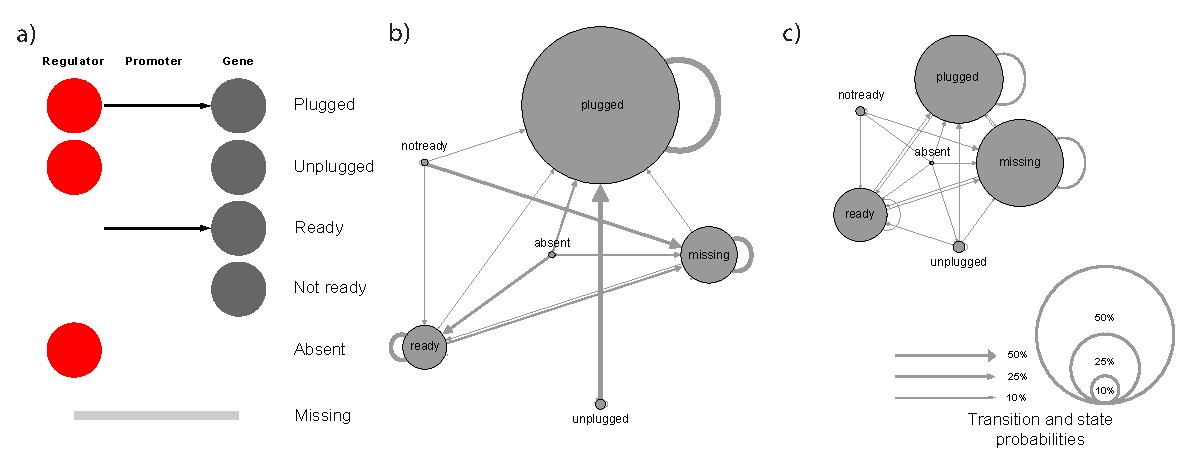
\includegraphics[width=0.8\textwidth]{./figures/Appendix_1/4_reg}
  	\caption{\label{fig:reg4} Regulatory network dynamics. a) Graphical representation of the six states in which each regulatory link (a gene found with a TFBS in at least one genome) can be found in the \textit{S. meliloti} species and between the outgroup species; b) states probabilities and states transitions probabilities inside the \textit{S. meliloti} species: nodes and edges sizes are proportional to the probability in the model; c) states probabilities and states transitions probabilities between the outgroup species}
\end{figure}%
 Then, each target gene can be found in one of six different states (Figure~\ref{fig:reg4} (a): the "plugged" state, the only functional one, which corresponds to a target gene with a TFBS in its promoter region and the TF present in the genome, and other five non-functional states.
 These states miss: i) the TFBS ("unplugged"), ii) the TF ("ready"), iii) both the TF and the TFBS ("not ready"), iv) the regulated gene ("absent") or v) both the TF and the gene itself ("missing").
This HMM can be used to estimate the probability for state transitions, that is the probability of observing a change from one state to another in time.
 Therefore, by looking at the transition probabilities modelled on our predicted regulatory networks we could get an insight on the evolutionary dynamics of the regulatory network, specifically how the gene regulatory network changes in evolution by adding or removing genes.

According to the model, the most represented state in the \textit{S. meliloti} regulatory network is the "plugged" one, indicating conservation of regulatory interactions at the species level (Figure~\ref{fig:reg4} (b) and Table SM3).
More interestingly, the model predicts that the most frequent way through which the regulatory network grows is through the recruitment of "unplugged" genes.
 Very little probability was given to the "plugged" to "missing" transition, indicating that genes belonging to the gene regulatory network are rarely removed from the genome.
 On the other hand, genes with no TFBS and its cognate TF were frequently found to result in the loss of the gene ("not ready" to "missing"), highlighting the importance of regulatory interactions for gene conservation at the species level.
 When considering a wider phylogenetic level (the outgroups), the broader variability in TF gene targets resulted in the "plugged" and "missing" state as equally probable, indicating that regulons might evolve by adding and removing new elements to a conserved kernel of gene targets (Figure~\ref{fig:reg4} (c) and Table SM3).
 This is also reflected in a smaller probability that a target gene i) remains in the "plugged" state when compared to the \textit{S. meliloti} species level, and ii) acquires a TFBS.
 On the other hand, the same probability as inside \textit{S. meliloti} species was observed for the transition "not ready" to "missing", which seems to confirm the importance of regulatory features in explaining the dispensable genome evolution.
 Consequently, a striking different dynamics of regulatory circuitry evolution seems to be present in relation to the taxonomic ranks; at the species level, robust networks are formed and they tend to include new genes from the species pangenome, which then may be fixed if they provide a fitness gain.
On the contrary, when comparing wider taxonomic ranges, regulatory networks are less conserved and apparently genes are included in each species' genome directly with their regulatory features (in a sort of “plug-and-play” model).
% However, we cannot a priori exclude that some of these differences between intra- and inter-species evolutionary behaviour may be overestimated due to the lack of detailed information on the outgroups TFBS.

\subsubsection{Replicon-specific regulation and cross-regulation}
Transcription factors with replicon preference were found to have functional signatures in accordance with the functions encoded in the three main replicons of \textit{S. meliloti}.
 Using a clustering approach on normalized gene hits on each replicon we have found that 19 TFs preferentially regulate genes belonging to one of the three replicons: five to the chromosome (NtrR, OxyR, NesR, ChvI and SMc03165), six to the pSymB chromid (SM-b21706, SM-b20667, ChpR, RbtR, SM-b21598 and SM-b21372) and eight to the symbiotic megaplasmid pSymA (SyrM, NodD3, RhrA, NodD1, NodD2, FixJ, FixK1 and NifA) (Figure~\ref{fig:reg5} (a)); these TFs are also encoded by the same replicon. %
\begin{figure}[!tb]
	\centering
	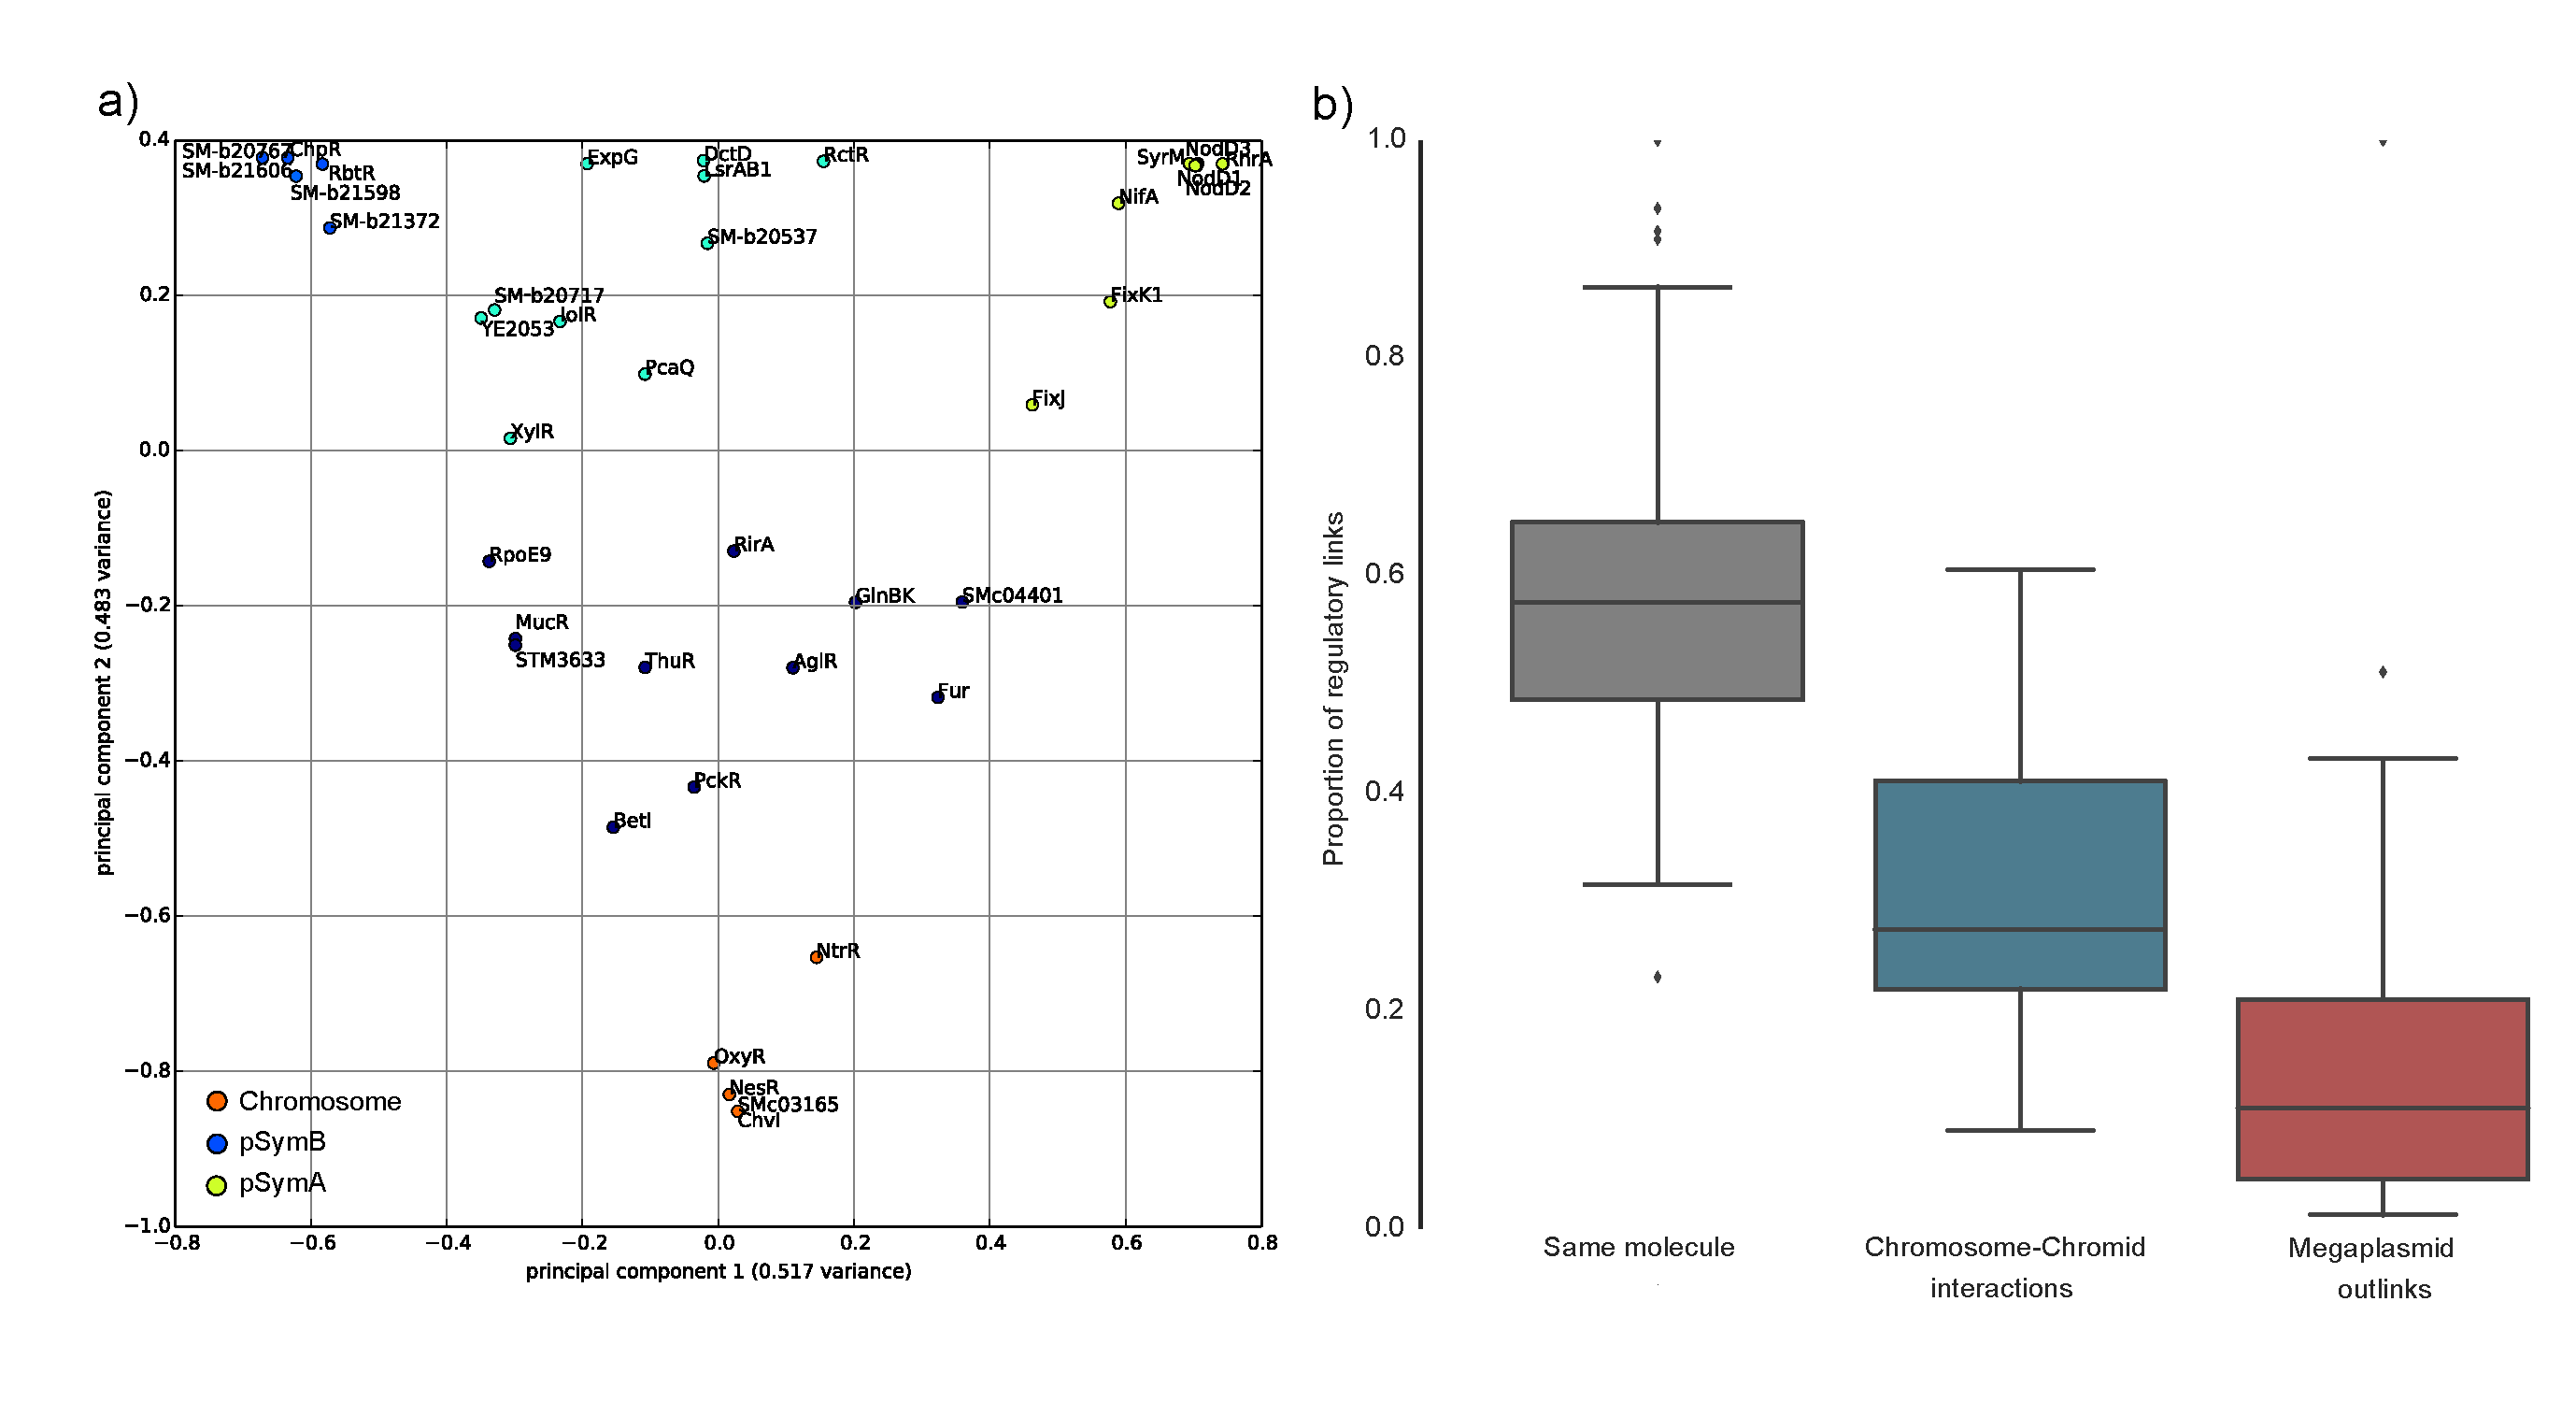
\includegraphics[width=1\textwidth]{./figures/Appendix_1/5_reg}
  	\caption{\label{fig:reg5} TFs preferentially associated with a replicon. a) K-means clustering of the normalized proportion of genes regulated in each replicon of \textit{S. meliloti}, visualized in a two-dimensional PCA; b) Variability in the number of regulatory links in the same replicon and between replicons. All differences are significant (t-test p-value $<$ 0.05)}
\end{figure}%
The six TFs located in the pSymB chromid (whose regulon is also preferentially located on pSymB) appear to mostly regulate the transport and metabolism of various carbon and nitrogen sources, including ribitol (RbtR), tagatose, sorbitol and mannitol (SM-b21372), ribose (SM-b21598), lactose (SM-b21706) and tartrate, succinate, butyrate and pyruvate (SM-b20667).
 The eight TFs present in the symbiotic megaplasmid pSymA (with regulons preferentially located on pSymA) were found to be involved in the regulation of key symbiotic processes, including nitrogenase synthesis and functioning through micro-aerophilia (FixJ, FixK1 and NifA), nod-factors biosynthesis (SyrM, NodD1, NodD2 and NodD3), and iron scavenging (RhrA).

A functional enrichment analysis using COG annotations (Figure SM3) on genes belonging to the regulons of the replicon-biased TFs confirmed this general observation: no functional category was enriched in the chromosome.
 The G category (\emph{carbohydrate metabolism and transport}) was enriched in genes regulated by pSymB encoded TFs, in agreement with the role of chromid pSymB in providing metabolic versatility to \textit{S. meliloti}.
 The C (\emph{energy production and conversion}), U (\emph{intracellular trafficing and secretion}) and T (\emph{Signal Transduction}) categories were enriched in genes under the control of pSymA-harboured TFs, which show some relationship with the establishment on the plant symbiosis.
 This analysis allowed us to depict a scenario where a significant part of the regulatory network is replicon-specific, with a tendency to maintain the functional signature of the host replicon, thus confirming earlier reports on the evolutionary independence of chromids and megaplasmids in \textit{S. meliloti} \cite{harrison2010introducing, galardini2013replicon}.

Interestingly, a fraction of TFs have target genes which span over different replicons, and show a preference for cross regulation between the chromosome and the chromid (Figure~\ref{fig:reg5} (b)).
The presence of cross-replicon regulons, may indeed allow a stabilization of genomic structure, genetically and metabolically connecting chromosome encoded functions with those present in the other two \textit{S. meliloti} replicons.
 In the evolutionary model of the chromid \cite{harrison2010introducing, galardini2013replicon, maclean2014examination}, the stabilization of the chromid into the host genome is related to the acquisition of essential (core) genes in a previously introgressed megaplasmid which gained niche-specific genes.
 Here we found that for TFs encoded on the chromosome (as AglR, GlnBK, IolR, BetI, LsrAB, MucR, PckR, RirA, NesR, RctR) a variable number of target genes are present on pSymB (Supplemental Material S1). The preference for cross-regulation between the chromosome and the chromid, as opposed to the megaplasmid uncovers an additional mechanism by which a chromid integrates itself in bacterial pangenomes.


\subsection{Discussion}

Regulatory networks are key components of cell's response to environmental changes. In the past years, several works have highlighted a high transcriptomic variability, in addition to genomic variation, in strains or individuals from the same species \cite{Cavalieri24102000, kvitek2008variations}.
Consequently, regulatory network variation can have profound impact on local adaptation and fitness of organisms. Recent studies have confirmed that bacterial regulatory networks are able to tolerate the addition of new genes in the transcriptional network \cite{isalan2008evolvability}, which in turn can serve as raw material for selection to operate. Using our original combined search strategy, we indeed found variability in regulon composition within the \textit{S. meliloti} species, which in fact accounted on average on 40\% of the regulon of each strain. On the other hand the regulon size was found to be conserved even outside the species boundary. This could suggest that even though the genes under the control of a TF vary between strains, there is a general constraint on the size of the transcriptional response. Whether this is due to energy constraints or simply an effect due to the genome base composition is yet to be clarified. 

The regulatory network distance (as defined in \cite{babu2006evolutionary}) correlates with upstream regions sequence divergence and patterns of genes presence/absence in the dispensable genome suggest that they both influence the regulatory network composition; the sequence divergence in upstream regions can result in the appearance or disappearance of TFBS, thus changing the regulatory network content. The genes presence/absence patterns in the dispensable genome can also have a strong impact on the regulatory network, with the introduction of new genes with a TFBS. This indicates that the evolution of bacterial regulatory networks, as that of the pangenome can be influenced by mechanisms of gene acquisitions, such as lateral gene transfer, and it's not only linked to gradual mutations in upstream regions.

The evolutionary dynamics of the regulatory network demonstrates the presence of selective pressures that govern gene presence/absence patterns in the dispensable genome. Indeed, even if a significant difference in the state transitions of regulatory links inside and outside the species boundary has been shown,  we have observed a similar tendency to disappear from the pangenome for genes that lack both a TFBS and its cognate TF. This indicates that the dynamics governing pangenome evolution may not be neutral, but also depend on the presence of those genes inside the regulatory network. In fact, fit of theoretical models to the pangenome of several bacterial species has already confirmed that pangenome evolution is under selective pressures \cite{lobkovsky2013gene}; we suggest that regulatory networks have an important role in shaping the bacterial gene content and contribute to genes fitness, which in turn may be linked to environmental adaptation. 

Moreover, the preference of nineteen TFs for target genes on one of the three replicons of \textit{S. meliloti} indicates that in multipartite bacterial genomes, similarly to replicon-dependent patterns of evolution in gene and functions content \cite{galardini2013replicon}, a replicon-specific transcriptional regulation is to be expected. At the same time, a significant number of cross-links between the chromosome and the chromid uncovers an for the first time an additional mechanism by which new replicons integrate into a bacterial pangenome.

% You may title this section "Methods" or "Models". 
% "Models" is not a valid title for PLoS ONE authors. However, PLoS ONE
% authors may use "Analysis" 
\subsection{Materials and Methods \label{sec:mat}}

\subsubsection{Genome sequences}
The 51 genomic sequences belonging to \textit{Sinorhizobium meliloti} and the five genomic sequences from closely related symbiotic species are listed in Table SM4.

\subsubsection{Orthology}
The orthology relationships inside the 51 \textit{S. meliloti} strains has been computed using the Blast-BBH algorithm implemented in the DuctApe suite (version 0.13.0)\cite{galardini2014ductape}, using default parameters. The same analysis has been conducted on the five closely related species with the addition of the Rm1021 reference strain, using the BLOSUM62 scoring matrix to account for their greater sequence diversity.

\subsubsection{Regulators estimation}
The number of regulators present in each genome has been estimated using COG annotations. The similarity of each protein against the COG database has been measured with a rpsblast scan \cite{altschul1990basic}, using an E-value threshold of 1e-10. Each protein mapped to the COG category K (Transcription) has been considered as a putative regulator.

\subsubsection{Regulatory motifs collection}
The 83 regulators whose PSSM has been extracted are listed in Table SM1. For those motifs retrieved from the literature, we collected the upstream regions of the regulated genes and (when available), the consensus binding sites from bibliographical records; the upstream regions have then been analysed with the \textit{meme} program \cite{bailey2009meme}(version 4.9.0), using the model that retrieved the PSMM with higher similarity to literature. Twenty-two motif files have been generated using the information retrieved from the RhizoRegNet database \cite{krol2011rhizoregnet}. Fifteen motif files have been generated using the information retrieved from the RegTransBase database \cite{kazakov2007regtransbase}. For the 5 regulators having more than one predicted motif, for instance those having a variable length (FixJ, RpoD, RpoE2, RpoH1 and RpoH2), one motif file for each motif length has been generated.
All the retrieved motifs have been converted to HMM models using the \textit{hmmbuild} program from the HMMer suite \cite{eddy2009new, johnson2010hidden, eddy2011accelerated}(version 3.1b1), using the alignments present in the MEME motif file.
It has been previously shown that in bacterial genomes TFBS can be reliably distinguished from background DNA only if their information content is higher than the minimum information content for the target genome, which depends on the genome size and composition \cite{wunderlich2009different} (this simplification of course ignores other factors such accessibility or proximity of the RNA polymerase). The information gain of the TFBS with respect to the genome is calculated using the Kullback-Leibler divergence between the corresponding nucleotide frequencies \cite{berg1987selection}, and it has been shown to correlate with the motif length and base composition of the motif with respect to the surrounding genome sequence. TF motifs with sufficient information content also tend to show less variability in their regulon composition between species \cite{quinn2014bacterial}; by focusing our analysis on such TFs we ensured a more precise analysis.
The information content of each motif has been calculated as suggested by Wunderlich et al \cite{wunderlich2009different}, using the Rm1021 reference genome for the calculation of the minimum information content; given the dependence of this variable on genome size and the fact that all the \textit{S. meliloti} strains have similar genome size, there has been no need to calculate a strain specific threshold. Motifs whose information content was found to be lower the minimum information content have been discarded with exception of FixJ, which has two distinct PSSM, one of which is above the threshold. In the presence of more than one source for a regulator (literature, RhizoRegNet or RegTransBase), the motif file having the highest information content has been considered in the final analysis.

\subsubsection{Search of regulatory motifs occurrences}
For each genome, background k-mers frequencies have been calculated using the \textit{fasta-get-markov} program from the MEME suite (version 4.9.0)\cite{bailey2009meme}, using 3 as the maximum value for k.
Each regulatory motif has been searched inside each genomic sequence using four scanning algorithms. The \textit{mast} program from the MEME suite (version 4.9.0)\cite{bailey2009meme} has been used with an E-value threshold of 100 and the use of a genome-specific background file. The \textit{matrix-scan} program from the RSAT suite \cite{van2003regulatory, thomas2008rsat, thomas2011rsat} has been used with a P-value threshold of 0.001, the background file and a pseudocount of 0.01, as suggested by Nishida et al. \cite{nishida2009pseudocounts}. The \textit{Bio.motifs} package from the Biopython library (version 1.62b)\cite{cock2009biopython} has been used with a false negative rate threshold of 0.05 and a pseudocount of 0.01, as suggested by Nishida et al. \cite{nishida2009pseudocounts}. The \textit{nHMMer} program from the HMMer suite (version 3.1b1)\cite{eddy2009new, johnson2010hidden, eddy2011accelerated} has been used with an E-value threshold of 100 and with all the heuristic filters turned off.
Each regulatory motif hit has been parsed, separating the hits being present in the upstream region of a gene from the others. The upstream region has been defined as the intergenic region in front of the first codon with a maximum size of 600 bp. In the case of a palindrome motif, the motif orientation has been ignored.

The distributions of the raw scores has been tested using a normality test, as implemented in the SciPy library (version 0.13.3)\cite{d1971omnibus}\cite{jones2001scipy}. The score threshold has been determined through the calculation of the raw scores quartiles (Q1 and Q3) and defining the score threshold ($\tau_S$ in Eq. \ref{scoreT}) in order to consider only the upper outliers \cite{hojo1931distribution}.

\begin{equation}
\label{scoreT}
\tau_S= Q3 + (1.5 (Q3-Q1)).
\end{equation}


For the Biopython method the bit score has been used, while for the RSAT, HMMer and MEME methods the negative base 10 logarithm of the E-value has been considered. The regulatory motifs predicted by at least three methods have been considered for further analysis. 

\subsubsection{Experimental confirmation of pomoters}
Upstream sequences from selected putative target genes of NodD regulon were analysed (see Table SM2). Sequences (approximately 400 nt upstream the translation start site of the gene) were amplified from crude lisates of \textit{S. meliloti} strains and cloned into pTO2 vector (which carries GFPuv as reporter gene \cite{karunakaran2005family}) by using  \textit{SalI} and  \textit{KnpI} restriction sites. Recombinant clones of \textit{E. coli} S17-1 strain were selected by gentamycin resistance and verified by sequencing of inserted fragments. Positive clones were used for transferring recombinant pOT2 vectors to  \textit{S. meliloti} Rm1021 by bi-parental conjugation by using previously described protocols \cite{pini2014molecular}\cite{pini2013divj}. \textit{S. meliloti} Rm1021 recombinant strains were then tested for GFP fluorescence after incubation of a 5 ml culture grown at the mid-exponential phase with 1 microM luteolin (Sigma-Aldrich) in liquid TY medium at 30$^{\circ}$C for 3h. GFP fluorecence was measured on a Infine200 Pro plate reader (Tecan). Measures were taken in triplicate and normalized to cell growth estimates as absorbance to 600nm.

\subsubsection{Operon prediction}
The operons belonging to the 56 genomes of this study have been predicted using the operon prediction software (version 1.2)\cite{westover2005operon}, using a beta threshold of 0.7 and a probability threshold of 0.5. The number and length of the predicted operons in each strain are listed in Table SM5.

\subsubsection{Replicon mapping}
Each contig of the 44 \textit{S. meliloti} draft genomes has been mapped to the seven complete genomes using CONTIGuator (version 2.7.3)\cite{galardini2011contiguator}, using a 15\% coverage threshold and considering blast hits over 1000 bp in length. A contig has been considered mapped to a replicon When it has been found mapped to the replicon in at least five complete genomes, or when it has been mapped to the replicon in at least one complete genome and to no replicon in the others.

The number of average gene hits have been divided for each replicon (either from a complete genome or a draft genome) and normalized by the number of genes belonging to each replicon in the Rm1021 reference strain. Regulators with preferential regulatory hits in a specific replicon have been highlighted performing a k-means clustering (k=5, selected using an elbow test \cite{ward1963hierarchical}) and plotted using the two principal components of the proportion of hits in each repliconusing the scikits-learn package (version 0.14.1)\cite{pedregosa2011scikit}. Only the three main replicons (chromosome, pSymB and pSymA) have been considered. COG categories enrichment have been tested using a Fisher's exact test, as implemented in the DendroPy package \cite{sukumaran2010dendropy}.

\subsubsection{Phylogenetic distance}
Phylogenetic distance inside the \textit{S. meliloti} pangenome and the pangenome of the five related species has been computed as described in a previous work \cite{galardini2013replicon}. The pangenome has been divided in three fractions, allowing the use of three distinct phylogenetic distances. The "core" distance has been calculated through the alignment of all the nucleotide sequences of each core gene, discarding those genes where at least one sequence was 60bp shorter or longer with respect to the other sequences. The "upstream" distance has been calculated through the alignment of the core genes upstream regions, discarding sequences below 5bp in length. The alignments have been calculated using MUSCLE (version 3.8.31)\cite{edgar2004muscle} and the bayesian tree has been inferred using MrBayes (version 3.2.0)\cite{ronquist2012mrbayes}. The distance matrix for both distance categories has been computed from the phylogenetic tree using the textit{Bio.Phylo} package inside the Biopython library (version 1.62b)\cite{talevich2012bio}. The "accessory" distance has been calculated through the construction of a presence/absence binary matrix for all the dispensable genome OGs; the distance between each strain has been then calculated using the Jaccard distance measure, as implemented in the SciPy library (version 0.13.3)\cite{jones2001scipy}.

\subsubsection{Regulatory network distance}
The distance between each strain inside the \textit{S. meliloti} and the other five related species regulatory network has been computed using the distance in the presence/absence of regulatory interactions as suggested in the work of Babu and collaborators \cite{babu2006evolutionary}. The distance between strain A and B is computed using Eq. \ref{babu}.

\begin{equation}D_{AB} = 1 - \cfrac{core_{AB}}{total_{AB}},
\label{babu}
\end{equation}

where $core_{AB}$ and $total_{AB}$ represent the number of conserved and total regulatory interactions, respectively.

Pearson and Spearman correlation coefficients between the pangenome and the regulatory network distance have been calculated using the implementations of the SciPy library (version 0.13.3)\cite{jones2001scipy}, removing the outliers with mean absolute deviation $>$ 3.5.

\subsubsection{Regulatory network transistions}
The state transitions of the regulatory network has been inferred by encoding them in a hidden markov model. Each one of the regulatory links observed in at least one strain has been tested for their state in each organism, following the labelling of Figure~\ref{fig:reg4} (a). Specifically, each regulatory link in the network of each organism could belong to one of the following categories:

\begin{itemize}
\item \textbf{Plugged:} regulator, gene and TFBS present
\item \textbf{Unplugged:} regulator and gene present, TFBS absent
\item \textbf{Ready:} gene and TFBS present, regulator absent
\item \textbf{Not ready:} gene present, regulator and TFBS absent
\item \textbf{Absent:} regulator present, gene and TFBS absent
\item \textbf{Missing:} regulator, gene and TFBS absent
\end{itemize}

The hidden markov model has been constructed using the Baum-Welch algorithm \cite{jelinek1975design}, as implemented in the GHMM python library. Transitions probability between states has been inferred averaging 1000 HMMs, constructed through a randomization of organisms order. 

\subsubsection{Results analysis and visualization}
Regulatory motifs data has been analysed and visualized using the NumPy \cite{van2011numpy} and matplotlib \cite{hunter2007matplotlib} libraries inside the iPython environment \cite{perez2007ipython}. Regulatory networks have been built using the networkx library \cite{networkx} and visualized using Gephi \cite{bastian2009gephi}.

\subsubsection{Data and methods availability}
Genomic sequences, regulatory motif files and search and analysis scripts are available as separate git repositories. The rhizoreg repository (https://github.com/combogenomics/rhizoreg/tree/paper), contains the input data; the regtools repository (https://github.com/combogenomics/regtools/tree/paper) contains the main scripts used to conduct the analysis.


%%-----------
%% Backmatter
%%-----------
\backmatter
\chaptermark{Bibliography}
\renewcommand{\sectionmark}[1]{\markright{#1}}
\bibliographystyle{unsrt}                           %Use alpha codes for references
\sectionmark{Bibliography}
\addcontentsline{toc}{chapter}{Bibliography}        %Force addition of Bibliography to TOC    
\bibliography{References}